\documentclass[russian,10pt,a4paper]{article}

\usepackage[intlimits]{amsmath}
\usepackage{amsthm,amsfonts}
\usepackage{amssymb}
\usepackage{mathrsfs}
%\usepackage{graphicx}
\usepackage[final]{graphicx,epsfig} 
\usepackage{longtable}
\usepackage{indentfirst}
\usepackage[utf8]{inputenc}
\usepackage[T2A]{fontenc}
\usepackage[russian,english]{babel}
\usepackage[usenames]{color}


\pdfpagewidth 20cm


\hyphenpenalty=3000
\tolerance=3000

% Adjust first page number according to real document position in the book.
\setcounter{page}{1}

% Dot after section number
\makeatletter
% In section title
\def\@seccntformat#1{\csname the#1\endcsname.\quad}
\makeatother

%\tolerance = 2000

% To place author above title
\def\maketitle{
  \begin{center}
  
{\large Графмодели ДЗ № 2 } \\ 
Бузун Назар, postrealist@gmail.com
  \end{center}
}

\renewcommand{\refname}{Литература}

%\sloppy
%\DeclareGraphicsRule{*}{eps}{*}{}
\DeclareMathOperator{\diam}{diam}

\graphicspath{{images/}}
\newcommand{\imgh}[3]{\begin{figure}[!h]\center{\includegraphics[width=#1]{#2}}\caption{#3}\label{Fig:#2}\end{figure}}

% Perfectly typesetted tilde for url links.
%\def\urltilde{\kern -.15em\lower .7ex\hbox{\~{}}\kern .04em}

\addto{\captionsrussian}{
    \renewcommand{\proofname}{\bf Решение. }
}

\usepackage{wasysym}

\theoremstyle{definition}
%\newtheorem{problem}{\noindent\normalsize\bfЗадача \No\!\!}
\newtheorem{problem}{\noindent\normalsize\bf{}}[section]
\renewcommand{\theproblem}{\arabic{problem}}
\newtheorem{example}{\noindent\normalsize\bf{}Пример}
\newtheorem*{definition}{\noindent\normalsize\bf{}Определение}
\newtheorem*{remark}{\noindent\normalsize\bf{}Замечание}
\newtheorem{theorem}{\noindent\normalsize\bf{}Теорема}
\newtheorem{fixme}{\noindent\normalsize\bf{}\frownie{} fixme}
\renewcommand{\thefixme}{}

\newtheorem*{ordre}{\noindent\normalsize\bf{}Указание}

\newenvironment{solution}{\begin{proof}\vspace{1em}} {\end{proof} \vspace{2em}}

\usepackage{verbatim}



\usepackage{enumitem}

\RequirePackage{enumitem}
\renewcommand{\alph}[1]{\asbuk{#1}} % костыль для кирилической нумерации 

\setenumerate[1]{label=\alph*), fullwidth, itemindent=\parindent, 
  listparindent=\parindent} 
\setenumerate[2]{label=\arabic*), fullwidth, itemindent=\parindent, 
  listparindent=\parindent, leftmargin=\parindent}

\newcommand{\rg}{\ensuremath{\mathrm{rg}}}
\newcommand{\grad}{\ensuremath{\mathrm{grad}}}
\newcommand{\diag}{\ensuremath{\mathrm{diag}}}
\newcommand{\const}{\ensuremath{\mathop{\mathrm{const}}}\nolimits}
\newcommand{\Var}{\ensuremath{\mathop{\mathbb{D}}}\nolimits}
\newcommand{\Exp}{\ensuremath{\mathrm{{\mathbb E}}}}
\newcommand{\PR}{\ensuremath{\mathrm{{\mathbb P}}}}
\newcommand{\Be}{\ensuremath{\mathrm{Be}}}
\newcommand{\Po}{\ensuremath{\mathrm{Po}}}
\newcommand{\Bi}{\ensuremath{\mathrm{Bi}}}
\newcommand{\Ker}{\ensuremath{\mathrm{Ker}}}
\newcommand{\Real}{\ensuremath{\mathrm{Re}}}
\newcommand{\Lin}{\ensuremath{\mathrm{Lin}}}
\newcommand{\Gl}{\ensuremath{\mathrm{Gl}}}
\newcommand{\mes}{\ensuremath{\mathrm{mes}}}
\newcommand{\cov}{\ensuremath{\mathrm{cov}}}


\begin{document}

\selectlanguage{russian}
\maketitle

\section{Пояснения к методу сегментации}

Формула для ошибки, усредненной по классам, в терминах суперпикселей:  потеря на одном суперпикселе (loss) равна 
\begin{enumerate}
\item При $\widehat{y}_i = y_i$:  1/2 * количество левых пикселей в суперсикселе / количество пикселей в изображении того же гласа что и левые пиксели;
\item При $\widehat{y}_i \neq y_i$:  1/2 * количество доминирующих (по классу) пикселей в суперсикселе / количество пикселей в изображении того же гласа что и доминирующие пиксели.
\end{enumerate}


Решение задачи минимизации энергии, дополненной функцией потерь, при помощи алгоритма построения разреза графа:
\[
E_i(y_i) = w_{y_i}^T  x_i - \mathrm{loss}(y_i)
\]
\[
E_{ij}(y_i, y_j) = w_{y_i y_j}^T  e_{ij}, 
\]
где $x_{i}$ -- признаки вершины,  $e_{ij}$ -- признаки ребра.

\[
[i-src]_w = E_i(0) +  E_{i<j}(0, 0) 
\]
\[ 
[i-sink]_w = E_i(1) +  E_{i<j}(1, 0) + E_{k<i}(1, 1) - E_{k<i}(1, 0)  
\]
\[
[j-i]_w = E_{i<j}(1, 0) + E_{i<j}(0, 1) - E_{i<j}(1, 1) -E_{i<j}(0, 0) > 0  
\]



SVM struct отимизация: 

использовалась java библиотека JLIS c параметрами:
MAX\_SVM\_ITER = 1000, DUAL\_GAP = 0.07, check\_inference\_opt = false, C = 0.04, L2 norm.

JLIS имеет преимущества в сравнении с С++ реализацией -- параллельное решение задач минимизации энергии, удобная интеграция с другими частями алгоритма, проверка корректности задачи минимизации.    
К недостаткам можно отнести плохие критерии остановки, часто приводящие к зацикливанию, отсутствие документации, неразборчивый код.

\subsection*{Унарные признаки}

\[
f_i = ( \vec{x} \cdot [y_i = 0] , \vec{x} \cdot [y_i = 1] ) 
\] 

\subsection*{Парные признаки}

\[
f_{ij} = ( \vec{c_1} \cdot [y_i = 0, y_j = 0] , \vec{c_2} \cdot [y_i = 1, y_j = 1],  \vec{c_3} \cdot [y_i \neq y_j]) 
\] 

В качестве компонент векторов $\vec{c_1}$, $\vec{c_2}$, $\vec{c_3}$ можно брать следующие величины:

\begin{itemize}
\item $1.0$
\item длина границы
\item I(сила границы $> c$) 
\item max(сила границы, $c$) 
\item $\cos(x_i, x_j)$
\item $\exp(\gamma \Vert x_i -  x_j \Vert^2)$
\item $\vec{e_c}$ --  базисный вектор пары категорий соседних суперпикселей. Данный признак позволяет учесть какие объекты с сильно отличающимися признаками могут сочетаться а одном классе (например красные фары часто сочетаются и черным цветом остальных частей автомобиля). Для задания данной части парного признака было создано 10 категорий из унарных признаков при помощи метода weka.SimpleKMeans. Аналогичную кластеризацию можно было провести по усредненным RGB   цветам суперпикселей. 
\end{itemize} 

\section{Тестирование}


\imgh{80mm}{C}{Подбор параметра регуляризации по разбиению выборки на 2 блока.}

\imgh{80mm}{size}{Переобучение в зависимости от размера обучающей выборки.}

\imgh{80mm}{time}{Время работы в зависимости от размера обучающей выборки.}

Для итогового обучения были выбраны изображения с 1 по 100, остальные для проверки качества. Время работы: 1536 сек, средний loss на обучающей выборке 
0.117, средний  loss на тестовой выборке\textbf{ 0.123}.  


\begin{figure}[!h]
  \center
    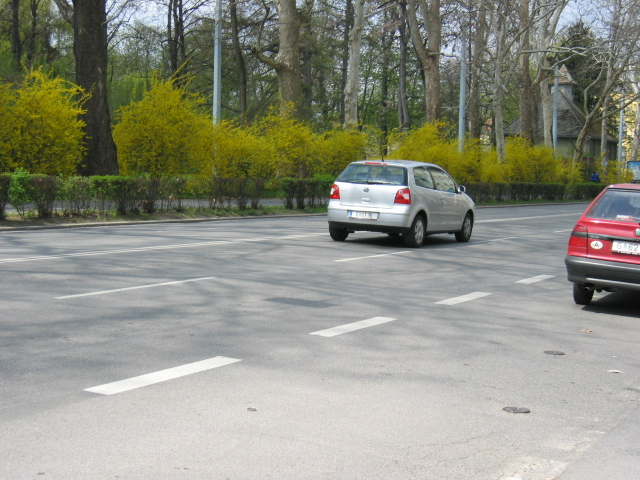
\includegraphics[width=0.45\linewidth]{images/imgTrain_110}$ $
    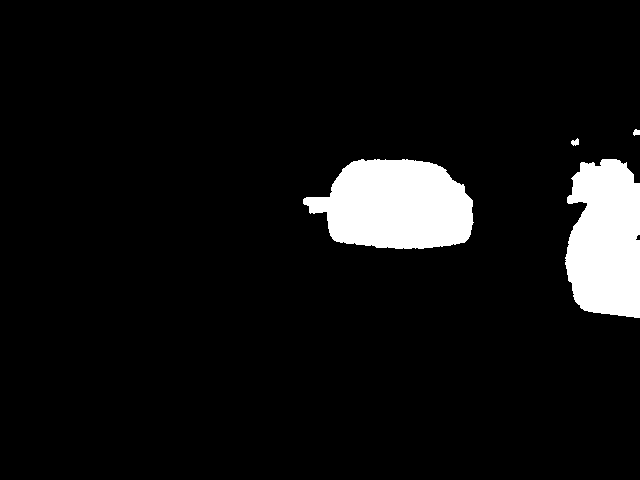
\includegraphics[width=0.45\linewidth]{images/110_segm_res}
loss=0.036
 
 \hfill

  \center
    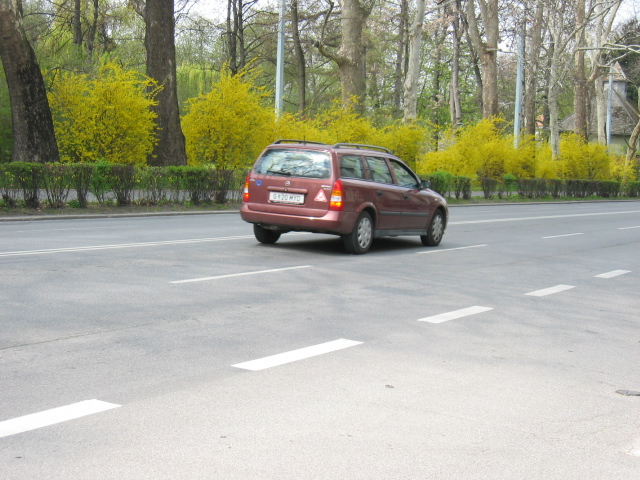
\includegraphics[width=0.45\linewidth]{images/imgTrain_111}$ $
    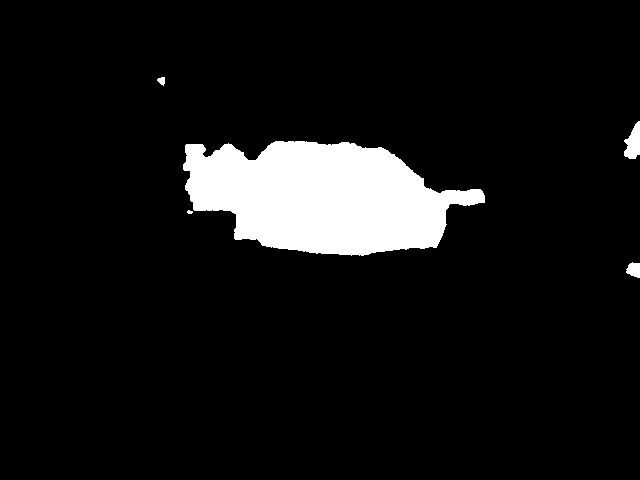
\includegraphics[width=0.45\linewidth]{images/111_segm_res}
loss=0.021
\end{figure}



\begin{figure}[!h]
  \center
    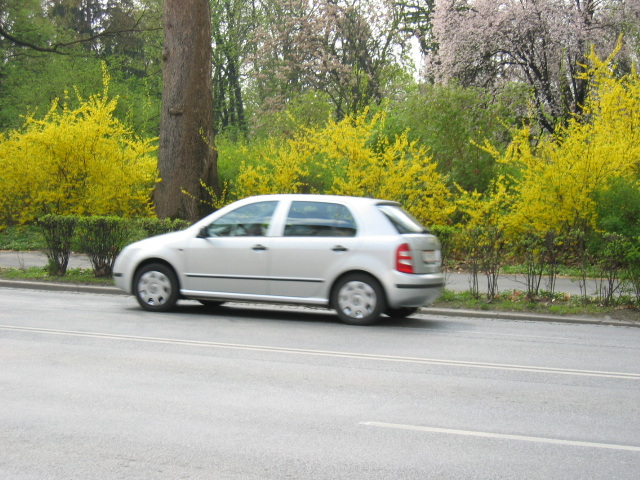
\includegraphics[width=0.45\linewidth]{images/imgTrain_112}$ $
    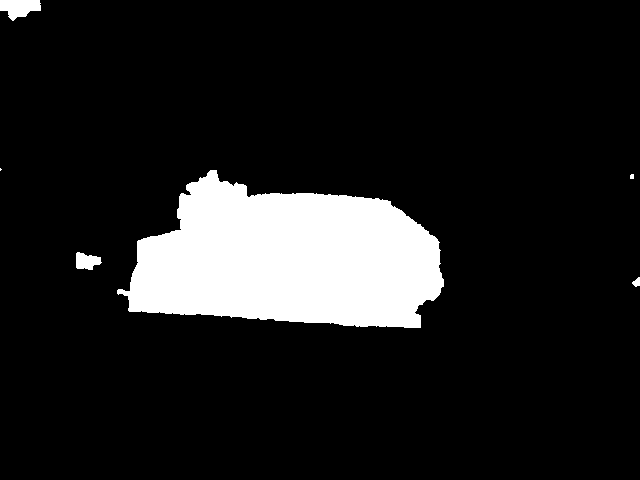
\includegraphics[width=0.45\linewidth]{images/112_segm_res}
loss=0.036
\end{figure}



\begin{figure}[!h]
  \center
    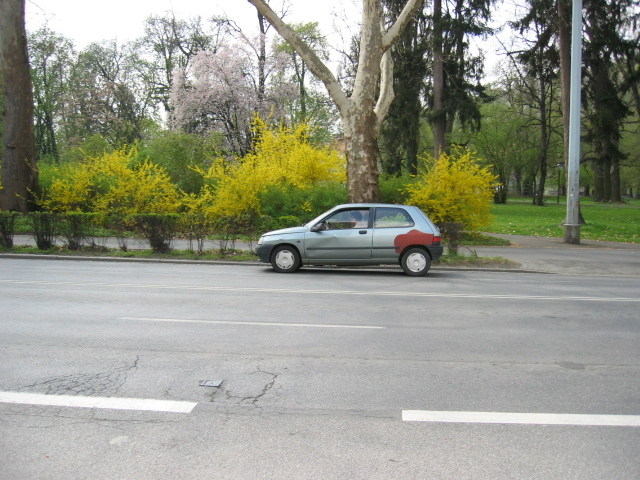
\includegraphics[width=0.45\linewidth]{images/imgTrain_113}$ $
    
\includegraphics[width=0.45\linewidth]{images/113_segm_res}
loss=0.031
\end{figure}



\begin{figure}[!h]
  \center
    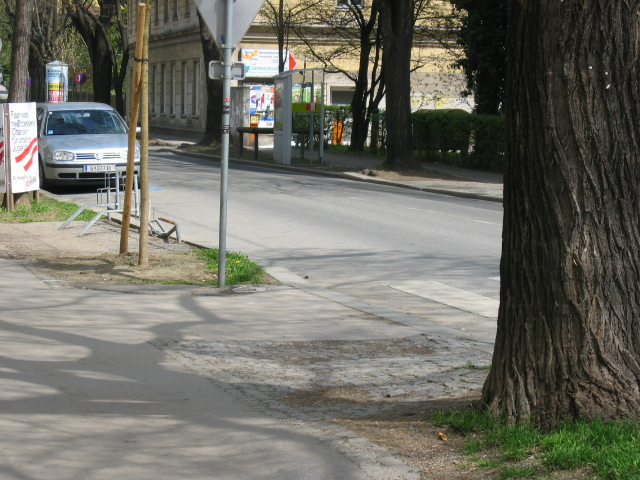
\includegraphics[width=0.45\linewidth]{images/imgTrain_143}$ $
    
\includegraphics[width=0.45\linewidth]{images/143_segm_res}
loss=0.198
\end{figure}

\begin{figure}[!h]
  \center
    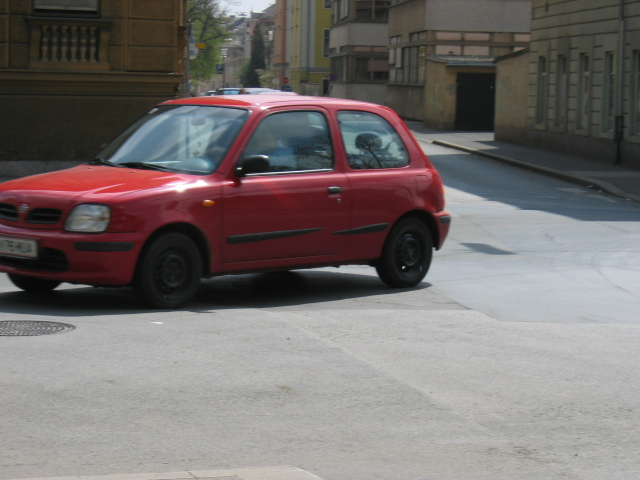
\includegraphics[width=0.45\linewidth]{images/imgTrain_144}$ $
    
\includegraphics[width=0.45\linewidth]{images/144_segm_res}
loss=0.119
\end{figure}


\begin{figure}[!h]
  \center
    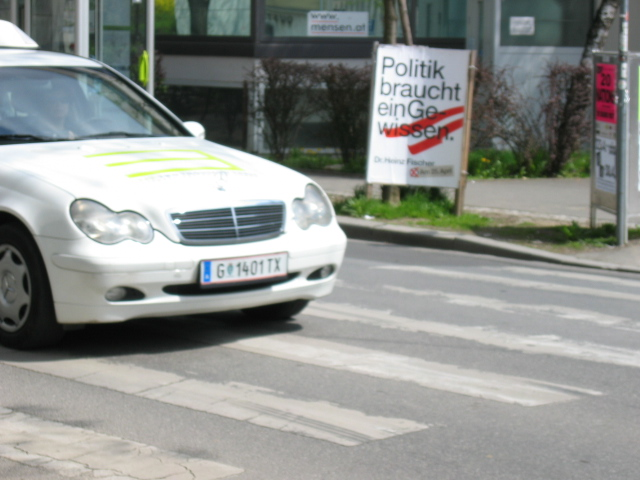
\includegraphics[width=0.45\linewidth]{images/imgTrain_145}$ $
    
\includegraphics[width=0.45\linewidth]{images/145_segm_res}
loss=0.139
\end{figure}


\begin{figure}[!h]
  \center
    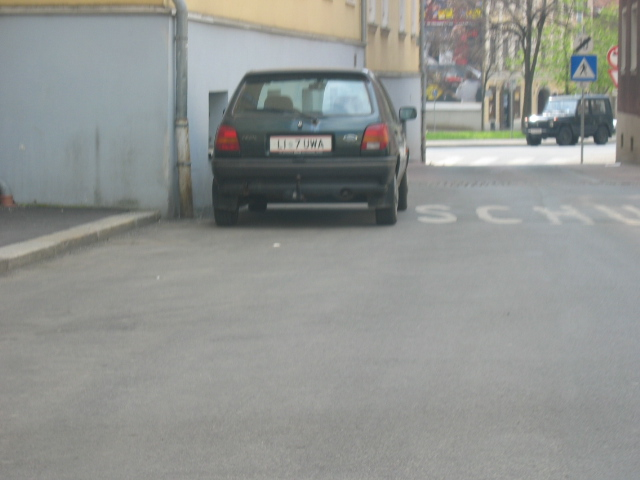
\includegraphics[width=0.45\linewidth]{images/imgTrain_146}$ $
    
\includegraphics[width=0.45\linewidth]{images/146_segm_res}
loss=0.152
\end{figure}


\begin{figure}[!h]
  \center
    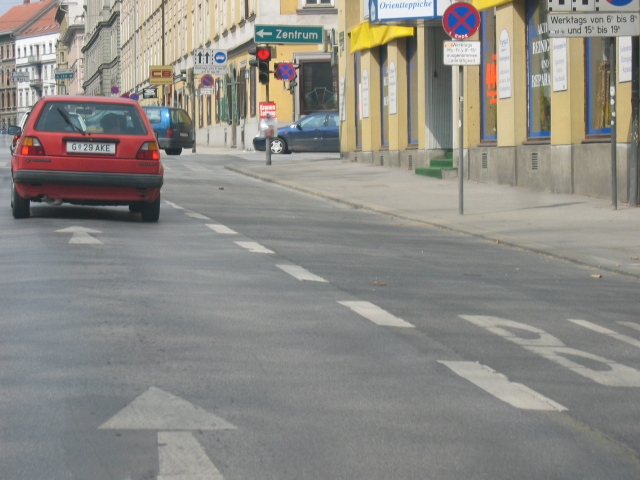
\includegraphics[width=0.45\linewidth]{images/imgTrain_147}$ $
    
\includegraphics[width=0.45\linewidth]{images/147_segm_res}
loss=0.234
\end{figure}


\newpage






\section{Резюме}

Минимизации энергии при помощи алгоритма построения разреза графа
кажется не самым удачным способом, так как очень часто удаление несубмодулярных ребер вносит значительное искажение в величину разреза по сравнения с энергией модели. Модно либо дополнить SVM struct дополнительным условием, либо использовать  MF Var Inference к примеру. 

При изменении параметра C и парных признаков оптимизация часто перестает сходится. Но при сильно заниженных С сходимость всегда есть.

По итогам сегментации: плохо выделяются машины малого размера, часто к машинам прилепляются куски фона, граница машины перестает быть гладкой и овальной, появляется много объектов ошибочно принятых за машину.  
       
\end{document}